% Define the document class. aastex for manuscript preparation, emulateapj for making it look polished.
% \documentclass[12pt,preprint2]{aastex}
%\documentclass[12pt,a4paper, iop,onecolumn,numberedappendix]{emulateapj}
\documentclass[12pt,preprint]{aastex}

% Import the natbib package for bibliography inclusion. To get it to work right, first typeset the bibliography (BibTex), Command-Shift-B.
% Then, typeset the document with LaTeX, Command-Shift-L or just Command-T.
% To get proper reference citations using aastex (preprint manuscripts), first typeset as emulateapj with BibTex to create the BibTex 
% files and then typeset again as aastex to get the manuscript with references.
\usepackage{natbib}
\usepackage{epsfig,graphicx,color}
\usepackage{longtable}

\bibliographystyle{apj}
% A few colors to replace the defaults for certain link types
\definecolor{orange}{cmyk}{0,0.4,0.8,0.2}
\definecolor{darkorange}{rgb}{.71,0.21,0.01}
\definecolor{darkgreen}{rgb}{.12,.54,.11}

%-----------------------------------------------------------------------------
% The hyperref package gives us a pdf with properly built
% internal navigation ('pdf bookmarks' for the table of contents,
% internal cross-reference links, web links for URLs, etc.)
\usepackage{hyperref}
\hypersetup{pdftex,  % needed for pdflatex
  breaklinks=true,  % so long urls are correctly broken across lines
  colorlinks=true,
  urlcolor=blue,
  linkcolor=darkorange,
  citecolor=darkgreen,
  }

%Define this shorthand for scientific notation.
\newcommand{\expnt}[2]{\ensuremath{#1 \times 10^{#2}}}   % scientific notation
\newcommand{\x}{{\bf x}}
\newcommand{\X}{{\bf X}}
\newcommand{\y}{{\bf y}}
\newcommand{\z}{{\bf z}}
\newcommand{\new}{red}
\newcommand{\ptr}{p_{\rm tr}}
\newcommand{\pte}{p_{\rm te}}
\newcommand{\Ex}{\mathbf{E}}
\newcommand{\Prob}{\mathbf{P}}
\newcommand{\PrfL}{\widehat{P}_{\rm{RF,}\mathcal{L}}(y|\x)}
\newcommand{\PrfLx}{\widehat{P}_{\rm{RF,}\mathcal{L}\cup\x'}(y|\x)}
\newcommand{\TreeL}{\theta_{b, \mathcal{L}}(y|\x)}
\newcommand{\TreeLx}{\theta_{b, \mathcal{L}\cup\x'}(y|\x)}
 \def\hipp {{\it Hipparcos~}}

\newcommand{\dd}{\mathrm{d}}

% Commands for annotating the docs with fixme and inter-author notes.  See
% below for how to disable these.
%
% Define a \fixme command to mark visually things needing fixing in the draft,
% as well as similar commands for each author to leave initialed special
% comments in the document.
% For final printing or to simply disable these bright warnings, symlink
% (there's a target 'dist_on' in the makefile that does this) the file
% macros_state.tex to macros_off.tex

\newcommand{\fixme}[1] { \textcolor{red} {
{\fbox{ {\bf FIX}
\ensuremath{\blacktriangleright \blacktriangleright \blacktriangleright}}
{\bf #1}
\fbox{\ensuremath{\blacktriangleleft \blacktriangleleft \blacktriangleleft}
} } } }

% And similarly, one (less jarring, with fewer symbols and no boldface) command
% for each one of us to leave comments in the main text.
\newcommand{\james}[1] { \textcolor{blue} {
\ensuremath{\blacklozenge} {\bf james:}  {#1}
\ensuremath{\blacklozenge} } }

\newcommand{\hogg}[1] { \textcolor{darkorange} {
\ensuremath{\blacksquare} {\bf hogg:}  {#1}
\ensuremath{\blacksquare} } }

\newcommand{\dan}[1] { \textcolor{darkgreen} {
\ensuremath{\bigstar} {\bf dan:}  {#1}
\ensuremath{\bigstar} } }

\newcommand{\joey}[1] { \textcolor{red} {
\ensuremath{\clubsuit} {\bf joey:}  {#1}
\ensuremath{\clubsuit} } }%\documentclass[manuscript]{aastex}


\begin{document}
%%%%%%%% TITLE, AUTHORS, PUBLICATION STATUS, and ABSTRACT %%%%%%%%%

\shorttitle{Fitting the Undetected}
\shortauthors{}
\title{Fitting the Undetected:  Light-curve Feature Estimation in the Presence of Non-detections}
\author{
Some wild \& crazy guys
}
%
%\altaffiltext{1}{Astronomy Department, University of California, Berkeley, CA, 94720-7450, USA}
%\altaffiltext{2}{Statistics Department, University of California, Berkeley, CA, 94720-7450, USA}
%\altaffiltext{*}{E-mail: {\tt jwrichar@stat.berkeley.edu}}

% Note the status (in preparation, MNRAS submitted date, ApJ accepted date, in press etc).
\slugcomment{in preparation}


\begin{abstract}
In multi-epoch imaging surveys, faint variable sources will not be
detectable at all epochs.  In principle, the best approach is to
perform photometric measurements anyway, so that there is a datum
recorded at at every epoch.  In practice, most surveys only provide
detection upper limits at some epochs; in some not even upper
limits but just the information that the star was not observed.  Here
we demonstrate with real data on periodic variables from the All-Sky
Automated Survey (ASAS) that these non-detections are nonetheless useful in
fitting and parameter estimation; their inclusion improves both
precision and accuracy.  One novel aspect of this work is that we do
not require the data source to include accurate---or even
any---information about the uncertainty variances on detections or the
values of the upper limits; we find that we can model these as latent
variables, even when they are different at every epoch.  Using realistic
simulations of Mira variable stars, we obtain amplitude estimates that
are {\bf XXX\%} more accurate by incorporating the non-detections into
the analysis.  For  Mira and RR Lyrae variables observed by ASAS, our
method obtains a tighter period - amplitude relationship than the standard
technique.
\end{abstract}

%\keywords{stars: variables: general -- methods: data analysis -- methods: statistical -- techniques: photometric}

\section{Introduction}
\label{sec:intro}



Surveys working in real-time tend to analyze each image with an eye to populating databases quickly. Unless a particular region of the sky gets special treatment (such as it is a known place of interest), discovery of variability happens by comparison of flux values at the database level. Analysis on such databases of transient/variables thus deals with censored data where there is often less information available that there should be. Even then, we might be able to infer what the thresholds were based on S/N measurements of objects neighboring the source of interest.


\joey{What people actually do, what problems that could cause, and what people should do}

A photometric survey (think of it as operating in a single photometric
bandpass for now) scans over the celestial position of a particular
variable star  a large number of times $t_i$.  At each of these
times, the imaging data are analyzed by software, which
treats each scan as a \emph{completely independent} survey.  That is,
when analyzing the data from time $t_i$, none of the information from
any of the other times is used in any way.




At each time $t_i$, the star is either detected ($q_i=1$) by the
software or not ($q_i=0$).  When it is detected, the software returns
a (possibly bad) flux value $f_i$ and (likely bad) uncertainty
variance $s_i^2$.  When the source is \emph{not} detected ($q_i=0$),
nothing is reported---in this case, because the software is not
awesome, it doesn't see any reason to report anything at all, since on
the non-detect passes, it has no inkling that this patch of the sky is
interesting in any way.  Welcome to the desert of the real.

Beyond this, there are two additional issues.  The first is that each
night of imaging is different in an unreported and unknown way.  That
is, there is different transparency, sky brightness, and point-spread
function.  So the detection limit, or completeness level, or censoring
of the catalog is different every night.  The second issue is that
either because we are getting the data from a non-generous source, or
because the conditions change rapidly and unpredictably, we can't
analyze all the sources in a finite patch simultaneously.  For each
variable star of interest, we \emph{only} get the data on that star
itself.

\joey{RRL end at 120 kpc in Sesar et al. paper}

\joey{discuss in context of: parameter estimation (amplitude / period), discovery (we're gonna find a lot more variable sources if we take the non-detections into account), and classification; lossiness}

\joey{let's make a point to stress variable discovery}

\joey{Numbers of LCs affected: Stripe 82, ASAS}




\section{Method}
\label{sec:method}


To recap, all we get at each epoch $t_i$ is a bit $q_i$ and, when
$q_i=1$, two data $f_i$ and $s_i^2$.  We don't get any information
about the upper limits or detection thresholds at the times $t_i$ when
$q_i=0$, and we don't know anything about the data quality (catalog
veracity) at any epoch.  For notational convenience we assemble all
the data into an enormous set $D$ given by
\begin{eqnarray}\displaystyle
D &\equiv& \{D_i\}
\\
D_i &\equiv& (q_i, f_i, s_i^2)
\quad ,
\end{eqnarray}
where the $f_i$ and $s_i^2$ data will be randomly generated or
meaningless at times at which the $q_i=0$.

We don't have access to all the information we need to use responsibly
the detections and non-detections in model fitting and inference.  We
have to instantiate latent variables to stand in for the missing
information.  For example, since we don't know the censoring threshold
or completeness limit for any observation $i$, we have to make it a
model parameter $b_i$.  Because we don't believe the reported
uncertainty variances $s_i^2$, we have to add parameters that model
the departure of the true uncertainty variance $\sigma_i^2$ from the
reported variance, and so on.

For the limited purposes here, the variable star will be periodic with
angular frequency $\omega$.  The expected brightness $\mu_i$ of the
star at time $t_i$ will be given by a linear combination of periodic
functions something like
\begin{eqnarray}\displaystyle
\mu_i &=& \sum_k A_k\,x_k(t_i|\omega)
\quad ,
\end{eqnarray}
where the $A_k$ are coefficients and the $x_k$ are functions.  This
can be generalized easily.  In addition to this expected brightness,
we assume that there is some either model uncertainty or stochastic
variation, leading to a \emph{model variance} $s_\mu^2$ at each point
(assumed constant but easily generalized).

If a source is detected at epoch $t_i$, we assume that its observed
flux $f_i$ is related to the expected flux $\mu_i$ by a Gaussian with
variance that has measurement and model contributions
\begin{eqnarray}\displaystyle
p(f_i|q_i,\sigma_i,\theta,I) &=& \left\{\begin{array}{ll}
  1 & \mbox{for $q_i=0$} \\
  N(f_i|\mu_i,s_\mu^2+\sigma_i^2) & \mbox{for $q_i=1$}
\end{array}\right.\label{eq:poff}
\\
\theta &\equiv& (\omega, \{A_k\}, s_\mu^2, \cdots)
\\
I &\equiv& (\{t_i\}, \mbox{assumptions})
\quad ,
\end{eqnarray}
where we have made the prior information about observation times $t_i$
and other assumptions explicit in the prior information blob $I$, and
we have a parameter blob $\theta$, which we will specify completely
below.  Note that the flux datum is ignored when the source is
undetected.

Similarly for the reported uncertainty variance $s_i^2$.  We don't
assume that it is correct in any case, but when the source is
detected, we assume that it is connected to the true uncertainty
$\sigma_i$ by a probabilistic likelihood, also Gaussian
\begin{eqnarray}\displaystyle
p(s_i|q_i,\sigma_i,\theta,I) &=& \left\{\begin{array}{ll}
  1 & \mbox{for $q_i=0$} \\
  N(s_i|\sigma_i,v_\sigma) & \mbox{for $q_i=1$}
\end{array}\right.
\\
\theta &\equiv& (\omega, \{A_k\}, s_\mu^2, v_\sigma, \cdots)
\quad ,
\end{eqnarray}
where we have added a model parameter $v_\sigma$, which represents the
variance in the distribution of reported uncertainties given the true
uncertainty; implicitly $v_\sigma$ is a component of $\theta$.  Again,
we are ignoring the variance datum when the source is undetected.

Under the assumption that the inclusion (or not) of the source in the
catalog is based on (or very strongly related to) the measured flux
(rather than the true flux), the natural likelihood for the bit $q_i$,
on which the above likelihoods are conditioned is
\begin{eqnarray}\displaystyle
P(q_i|b_i,\sigma_i,\theta,I) &=& \left\{\begin{array}{ll}
  \displaystyle\int_{-\infty}^{b_i} N(f|\mu_i,s_\mu^2+\sigma_i^2)\,\dd f & \mbox{for $q_i=0$} \\
  \displaystyle\int_{b_i}^\infty N(f|\mu_i,s_\mu^2+\sigma_i^2)\,\dd f & \mbox{for $q_i=1$}
\end{array}\right.\label{eq:pofq}
\quad,
\end{eqnarray}
where the integrals end at an observed-flux limit $b_i$, which (as
mentioned above) is also a model parameter.  The motivation for this
expression is that it imagines all possible observations $f$ of the
star at time $t_i$ given the model and uncertainties, and finds the
fraction that would make the (imagined) detection cut.

We are going to product together these likelihoods (for $q_i$, $f_i$,
and $s_i^2$); this looks like it is using the flux twice, once in the
PDF for $f_i$ in expression (\ref{eq:poff}) and once in the
probability for $q_i$ in expression (\ref{eq:pofq}).  It is not,
however, because in the probability for $q_i$ the flux $f$ that
appears is an integration variable, not an observation or datum.  We
treat the detections or non-detections as being ``prior'' to the
measurement.  This is the weakest plank in our otherwise impenetrable
fortress of solitude.

We are going to treat the true detection limit $b_i$ for each
observation, and its true uncertainty $\sigma_i$---two parameters
\emph{per data point}---as nuisance parameters.  We want to
marginalize them out.  This requires priors on these.  Again we choose
Gaussians for simplicity, but let the means and variances of these
Gaussians be new model parameters---hyperparameters if you wish.
\begin{eqnarray}\displaystyle
p(D_i|\theta,I) &=&
  \int P(D_i|b_i,\sigma_i,\theta,I)\,p(b_i|\theta)\,p(\sigma_i|\theta)\,\dd b_i\,\dd\sigma_i
\\
p(D_i|b_i,\sigma_i,\theta,I) &=&
  P(q_i|b_i,\sigma_i,\theta,I)\,p(f_i|q_i,\sigma_i,\theta,I)\,p(s_i|q_i,\sigma_i,\theta,I)
\\
p(b_i|\theta) &=& N(b_i|B,V_B)
\\
p(\sigma_i|\theta) &=& N(\sigma_i|S,V_S)
\\
\theta &\equiv& (\omega, \{A_k\}, s_\mu^2, v_\sigma, B, V_B, S, V_S)
\quad,
\end{eqnarray}
where we have (at last) explicitly assembled all the variable-star
parameters and hyperparameters into the big parameter vector $\theta$.
The huge sets of nuisance parameters $\{b_i\}$ and
$\{\sigma_i\}$ don't remain, because by integration we
removed them.

Finally and it goes without saying that if we treat the data points as
independent (as we are free to do, given the non-awesomeness of the
software data source), we have that
\begin{eqnarray}\displaystyle
p(D|\theta,I) &=& \prod_i p(D_i|\theta,I)
\quad.
\end{eqnarray}
This is the likelihood for variable-star parameters given the entire
data set (all the measurements and non-detections of this star from
all the epochs, as delivered by the untrustworthy robots).  It
``correctly'' or at least ``justifiably'' uses all of the information
available, without making strong assumptions about the survey or its
veracity.


\subsection{Implementation}
\label{ss:implemenation}



\joey{Describe Python implementation here}




\section{Experiments}
\label{sec:experiments}


\subsection{Simulating Faint Mira Variables}
\label{ss:mirasim}

In this first experiment, we begin with a well-observed Mira variable from the ASAS Catalog of Variable Stars (ACVS, \citealt{acvs}) , ASAS 235627-4947.2.  This star has a pulsation period of 266.6286 days and a Lomb-Scargle amplitude of 2.38 mag (V band).  Note there are no non-detections in the ASAS light curve.

To simulate faint Mira stars from ASAS 235627-4947.2, we use the following procedure:
\begin{enumerate}
\item Convert the observed magnitudes, $m_i$, and errors, $s_{m,i}$ to fluxes, $f_i$ and flux errors, $s_{f,i}$ (we assume a V-band zero-point of $3.67\times10^{-9}$ erg/s/cm$^2$/\AA)
\item For a given flux dimming parameter, $d$, sample the new fluxes, $\tilde{f}_i$, from a Gaussian distribution centered around $f_i / d$ with standard deviation sampled from the empirical ASAS distribution of $s_{f,i} | f_i$. \joey{I found that relationship to be linear with a slope $\approx 1$, which is probably BS since the ASAS mag errors are all crap.  So I added a reference value to each flux error to ensure a mag limit $\approx$ 14.5 mag.}
\item Fluxes that are not at least 5$\sigma$ above zero are denoted as non-detections and their flux estimates (and errors) are censored.
\end{enumerate}
Folded light curves of ASAS 235627-4947.2, dimmed by four different values of $d$, are plotted in Figure \ref{fig:mirasim}.


\begin{figure*}
\begin{center}
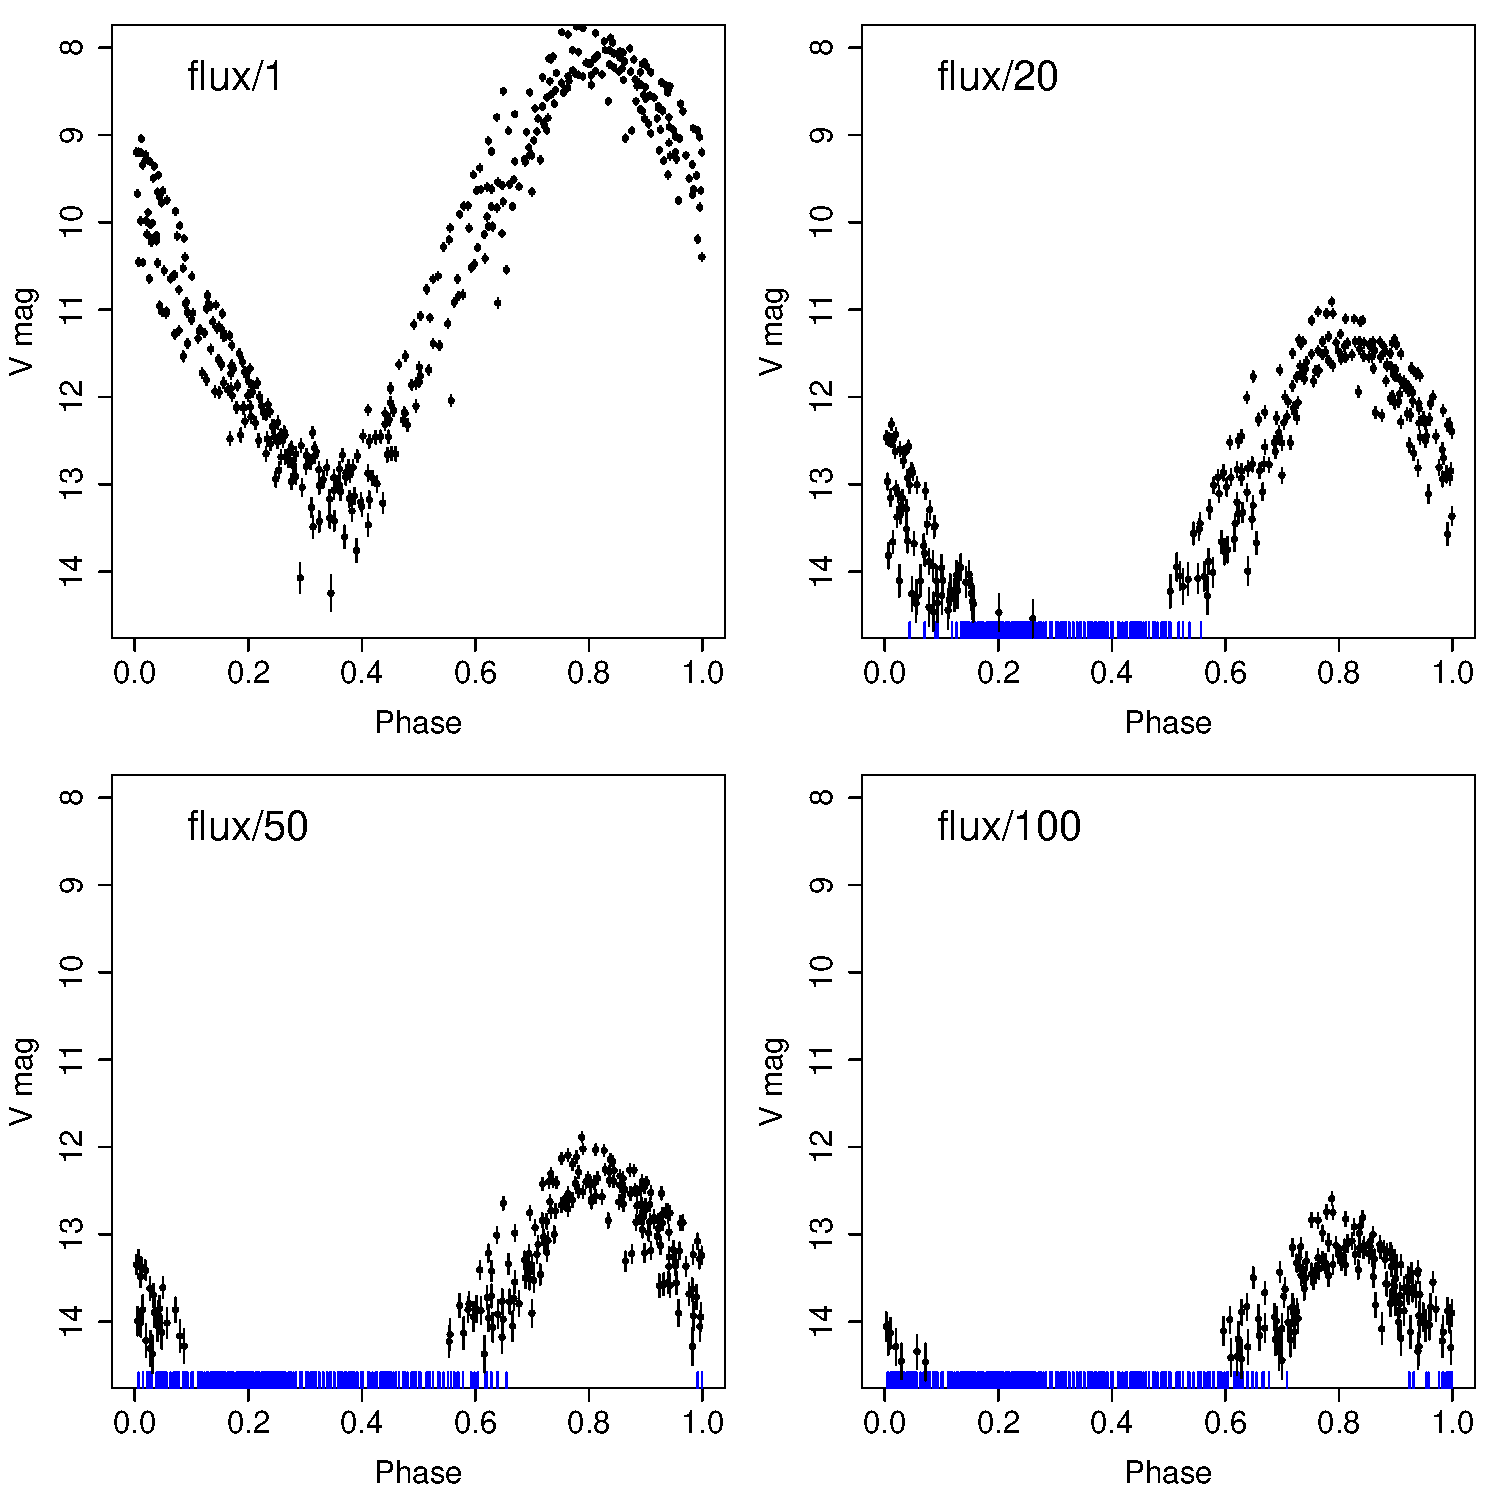
\includegraphics[angle=0,width=6.5in]{../plots/mira_simulated.pdf}
\end{center}
\caption{ Folded light curves for data simulated from the Mira variable ASAS 235627-4947.2 using the prescription in \S\ref{ss:mirasim}.  Blue tick marks along the bottom axis denote phases where there were non-detections.  As the original flux measurements are dimmed by higher factors, the troughs of the sinusoidal light curve are censored, resulting in an incomplete view of the data.  \label{fig:mirasim}}
\end{figure*}


\subsection{Results of Fitting Miras}


\section{Results: ASAS Light Curves}
\label{sec:results}

We use the methodology of \cite{2011arXiv1106.2832R} to select the top ASAS Mira  and RR Lyrae, Fundamental Mode candidates.  Using a posterior probability threshold of 0.8 gives us 1720 Mira  and 1029 RR Lyrae candidates.
 
 \subsection{Mira Variables}
 
 Show P - A relationship before and after using the method
 
 
 
 \subsection{RR Lyrae Variables}
 
  Show P - A relationship before and after using the method

There is an RRL P - A relationship (strong linear anti-correlation)
 

\section{Discussion}
\label{sec:discussion}

What people can do, starting from the data-taking procedure.

limitations



\acknowledgements


\bibliography{non_detect}

\end{document}
